\documentclass[paper=a4, fontsize=11pt]{scrartcl} % A4 paper and 11pt font size

\usepackage[T1]{fontenc} % Use 8-bit encoding that has 256 glyphs
\usepackage{fourier} % Use the Adobe Utopia font for the document - comment this line to return to the LaTeX default
\usepackage[english]{babel} % English language/hyphenation
\usepackage{amsmath,amsfonts,amsthm} % Math packages
\usepackage{graphicx}
\graphicspath{ {./images/} }
\usepackage{lipsum} % Used for inserting dummy 'Lorem ipsum' text into the template

\usepackage{sectsty} % Allows customizing section commands
\allsectionsfont{\centering \normalfont\scshape} % Make all sections centered, the default font and small caps

\usepackage{fancyhdr} % Custom headers and footers
\pagestyle{fancyplain} % Makes all pages in the document conform to the custom headers and footers
\fancyhead{} % No page header - if you want one, create it in the same way as the footers below
\fancyfoot[L]{} % Empty left footer
\fancyfoot[C]{} % Empty center footer
\fancyfoot[R]{\thepage} % Page numbering for right footer
\renewcommand{\headrulewidth}{0pt} % Remove header underlines
\renewcommand{\footrulewidth}{0pt} % Remove footer underlines
\setlength{\headheight}{13.6pt} % Customize the height of the header

\numberwithin{equation}{section} % Number equations within sections (i.e. 1.1, 1.2, 2.1, 2.2 instead of 1, 2, 3, 4)
\numberwithin{figure}{section} % Number figures within sections (i.e. 1.1, 1.2, 2.1, 2.2 instead of 1, 2, 3, 4)
\numberwithin{table}{section} % Number tables within sections (i.e. 1.1, 1.2, 2.1, 2.2 instead of 1, 2, 3, 4)

\setlength\parindent{0pt} % Removes all indentation from paragraphs - comment this line for an assignment with lots of text

%----------------------------------------------------------------------------------------
%	TITLE SECTION
%----------------------------------------------------------------------------------------

\newcommand{\horrule}[1]{\rule{\linewidth}{#1}} % Create horizontal rule command with 1 argument of height
\newcommand{\itab}[1]{\hspace{0em}\rlap{#1}}
\newcommand{\tab}[1]{\hspace{.2\textwidth}\rlap{#1}}

\title{	
\normalfont \normalsize 
\textsc{University of Maryland, Baltimore County} \\ [25pt] % Your university, school and/or department name(s)
\horrule{0.5pt} \\[0.4cm] % Thin top horizontal rule
\huge CMSC678 Homework 1  \\ % The assignment title
\horrule{2pt} \\[0.5cm] % Thick bottom horizontal rule
}

\author{Yin Huang} % Your name

\date{\normalsize\today} % Today's date or a custom date

\begin{document}

\maketitle % Print the title

%----------------------------------------------------------------------------------------
%	PROBLEM 1
%----------------------------------------------------------------------------------------

\section{Problem One}
In this part of the assignment you will gain familiarity with WEKA, the Waikato Environment for Knowledge Analysis. WEKA is widely used in the machine learning and data mining communities because, among other things, it provides both a nice user interface to a number of standard algorithms and a Java API.

First, you must download WEKA from the following URL: http://www.cs.waikato.ac.nz/ml/weka/. 

The "Getting Started" section of that page has links for information on system requirements, how to download the software, and documentation. WEKA is written in Java and should run on any platform with Java 1.5 or higher.

Read about the Adult Census Income dataset, and get it in the form of an ARFF file. Then do the following: 

\begin{itemize}
 \item  Build a decision tree (J48 classifier) with the default parameters and report the (stratified cross-validation) accuracy.
  \item  Now turn off pruning and report the accuracy. Inspect the output of the algorithm. Has it overfit? How can you tell?
  \item  Build a decision stump (a decision tree with a single split; you can find it in the tree section of algorithms in Weka) and report the accuracy. Inspect the output of the algorithm. Has it underfit? How can you tell?

\end{itemize}
%------------------------------------------------
\paragraph{Answer 1}
Below is the screen-shot of J48 classifier with the default parameters: \\
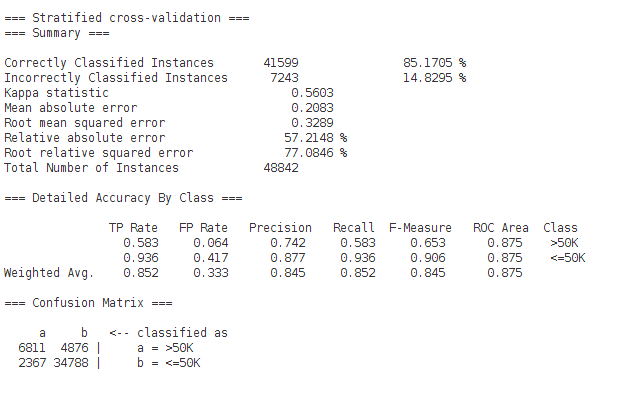
\includegraphics[scale=0.65]{question1.png}\label{Summary for default parameters J48 classifier} \\
Number of Leaves  : 	689   Size of the tree : 	834 
\paragraph{Answer 2}
Below is the screen-shot of J48 classifier without pruning: \\
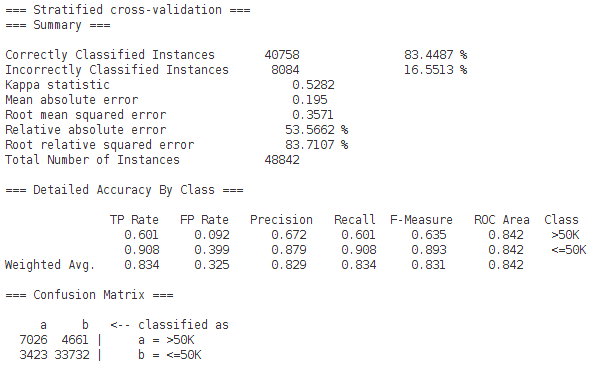
\includegraphics[scale=0.65]{question2.png}\label{Summary for default parameters J48 classifier without prunning} \\
Number of Leaves  : 	13074  Size of the tree : 	14871
Given the fact that the total size of the training set is 48842, and the output size of our decision tree is 14871 with 13074 leaves, we can safely assume this is overfitting because almost one quoter of our training set is used to build the decision tree. In a word, our tree has a high variance but low bias. In order to verify our assumption, we need to test the accuracy using other test data with no overlapping datasets with our training set.

\paragraph{Answer 3}
Below is the screen-shot of a decision dump with our dataset. 
\begin{center}
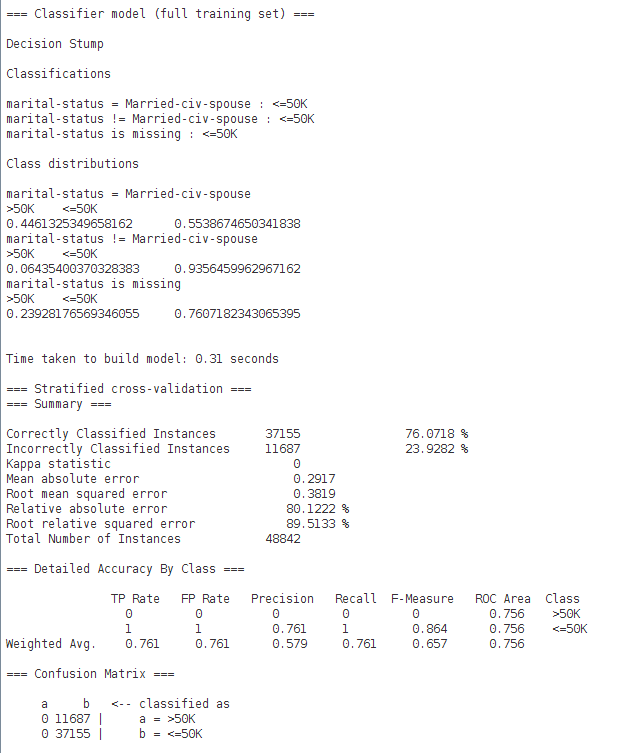
\includegraphics[scale=0.6]{question3.png}\label{Summary for a decision dump tree} \\
\end{center}
As we can see, the tree is only testing on one feature: marital-status and then give us the income label. This is absolutely underfitting since we have 15 attributes. In a word, our tree has a high bias but low variance. 

%----------------------------------------------------------------------------------------
%	PROBLEM 2
%----------------------------------------------------------------------------------------

\section{Problem Two}

%------------------------------------------------
In this part of the homework you will implement k-means clustering and experiment with different ways of initializing the cluster centroids.

The MNIST dataset is a well-studied collection of handwritten digits. It is often used to test multi-class classification algorithms, where there is one class for each of the 10 digits (0 - 9). In this homework, you will use it for unsupervised clustering.

I've made two files available for you: 
\begin{itemize}


  \item  The raw MNIST data, which is a text file containing 10,000 rows. Each row contains 28 * 28 = 784 integers in the range 0 to 255. Each integer is the pixel value from a 28 x 28 image of a handwritten digit. Every row corresponds to a vector in the dataset that is to be clustered.
  \item  The labels for the raw data are in a file with 10,000 rows. The first row contains the correct digit label for the first row in the raw data. The second row is the label for the second instance, and so on. 

\end{itemize}

 Implement the k-means clustering algorithm. You will only use your algorithm for this dataset, so you can hard-wire in the number of instances and the size of each instance.\\
 The goal is not to write a generic version of the algorithm (though you can if you wish). The goal is to understand how it works on real data. You will need to try different values of k so that must be a parameter.

After completing the implementation (and testing for correctness, of course), do the following: 
\begin{itemize}

 \item  Randomly sample k = 10 instances, use them as the initial cluster centroids, and run the algorithm to covergence. For each cluster, find the most common digit in that cluster and count the number of instances in the cluster that are different from the most common one. Sum that count over all of the clusters.
 \item   Repeat the above step 10 times in total and report the average number of iterations to convergence and the average number of instances that are in the wrong cluster.
 \item   Run the algorithm with k = 5. Look at the clusters and see if there are digits that tend to get grouped together. What are they and explain why you think they are grouped into the same cluster.
  \item  Finally, run the algorithm 10 times again with k = 10 and report the same information as above (iterations to convergence and number of wrongly clustered instances). But this time do not choose random instances for the cluster centroids. Randomly choose an instance that represents each of the digits and use them as the centroids. That is, one of the centroids will be a randomly chose 0, another will be a randomly chose 1, and so on. Do you observe any difference in the performance statistics? Why or why not?
 \item   Turn in hard copy of your code. 

\end{itemize}

\paragraph{Answer 1}
Randomly sample k=10 instances: \\

Exp Number:  1,2,3,4,5,6,7,8,9,10\\

Iteration numbers: 125, 56, 69, 55, 83, 53, 38, 92, 76, 69\\

Avg iteration number: 72 \\

Wrong instances: 4006,3942,4548,3936,4572,3947,4065,4013,4022,4057 \\

Avg wrong instances: 4111 \\
Ex 1 Most common digits: 3 1 0 8 7 6 4 7 2 1 \\
Ex 2 Most common digits: 6 0 2 5 7 8 1 3 4 7\\
Ex 3 Most common digits: 4 6 3 1 9 7 1 8 4 0\\
Ex 4 Most common digits: 3 0 9 4 2 6 7 1 8 5\\
Ex 5 Most common digits: 8 4 0 7 3 6 1 0 7 6\\
Ex 6 Most common digits: 7 3 2 1 8 4 7 6 0 0\\
Ex 7 Most common digits: 0 1 4 7 6 3 1 8 2 7\\
Ex 8 Most common digits: 3 1 6 2 0 7 8 4 1 7\\
Ex 9 Most common digits: 0 3 8 9 7 2 6 1 1 4\\
Ex 10 Most common digits: 2 7 3 0 9 1 1 8 6 4\\

Among all the most common digits: 1, 0, 7 are very common, 5, 9 are not common.\\

Avg computation time for one iteration: 40s\\

Initial center for the least iteration:\\
0 6 6 4 5 8 0 4 9 4 \\

Initial center for the most iteration:\\
9 8 3 8 7 0 4 1 2 7  \\
\begin{itemize}
	\item Exp 1:  \\
	
	Initials: [7380, 6935, 1067, 6435, 4297, 3140, 7421, 1633, 5717, 2332] \\
	
	Labels: [9 8 3 8 7 0 4 1 2 7 ] \\
	
    Total number of iterations: 125 \\
    
    Total running time is: 5083.837 s Average time is: 40.67s \\
    
    statistics: \\
   Cluster 1 has 1245 instances.\\
0 : 51  1 : 3   2 : 52  3 : 708 4 : 0   5 : 278 6 : 6   7 : 0   8 : 140 9 : 7\\
Most common digit is: 3 with 708 counts wrong instances: 537 counts\\

Cluster 2 has 723 instances.\\
0 : 1   1 : 485 2 : 119 3 : 4   4 : 9   5 : 17  6 : 8   7 : 45  8 : 32  9 : 3\\
Most common digit is: 1 with 485 counts wrong instances: 238 counts\\

Cluster 3 has 884 instances.\\
0 : 820 1 : 0   2 : 16  3 : 2   4 : 1   5 : 5   6 : 22  7 : 2   8 : 8   9 : 8\\
Most common digit is: 0 with 820 counts wrong instances: 64 counts\\

Cluster 4 has 1141 instances.\\
0 : 35  1 : 1   2 : 29  3 : 148 4 : 0   5 : 279 6 : 28  7 : 1   8 : 605 9 : 15\\
Most common digit is: 8 with 605 counts wrong instances: 536 counts\\

Cluster 5 has 1198 instances.\\
0 : 1   1 : 0   2 : 9   3 : 6   4 : 210 5 : 19  6 : 0   7 : 507 8 : 22  9 : 424\\
Most common digit is: 7 with 507 counts wrong instances: 691 counts\\

Cluster 6 has 897 instances.\\
0 : 28  1 : 2   2 : 23  3 : 5   4 : 20  5 : 12  6 : 798 7 : 0   8 : 7   9 : 2\\
Most common digit is: 6 with 798 counts wrong instances: 99 counts\\

Cluster 7 has 1065 instances.\\
0 : 3   1 : 0   2 : 26  3 : 14  4 : 441 5 : 42  6 : 14  7 : 138 8 : 25  9 : 362\\
Most common digit is: 4 with 441 counts wrong instances: 624 counts\\

Cluster 8 has 1117 instances.\\
0 : 32  1 : 0   2 : 18  3 : 14  4 : 273 5 : 205 6 : 19  7 : 293 8 : 96  9 : 167\\
Most common digit is: 7 with 293 counts wrong instances: 824 counts\\

Cluster 9 has 799 instances.\\
0 : 9   1 : 0   2 : 693 3 : 48  4 : 2   5 : 10  6 : 14  7 : 10  8 : 11  9 : 2\\
Most common digit is: 2 with 693 counts wrong instances: 106 counts\\

Cluster 10 has 931 instances.\\
0 : 0   1 : 644 2 : 47  3 : 61  4 : 26  5 : 25  6 : 49  7 : 32  8 : 28  9 : 19\\
Most common digit is: 1 with 644 counts wrong instances: 287 counts\\
Average wrong instances in this execution are: 4006 counts \\

\item Exp 2: \\

[7177, 2598, 3359, 9401, 1616, 2431, 5633, 6592, 2452, 8141] \\

[4 8 0 1 6 3 5 9 5 4 ] \\

Total number of iterations: 56\\

Total running time is: 2266.759 s Average time is: 40.47783928571429s\\

statistics: \\

Cluster 1 has 787 instances.\\
0 : 19  1 : 3   2 : 20  3 : 3   4 : 16  5 : 12  6 : 707 7 : 0   8 : 6   9 : 1\\
Most common digit is: 6 with 707 counts wrong instances: 80 counts\\

Cluster 2 has 803 instances. \\
0 : 747 1 : 0   2 : 12  3 : 1   4 : 1   5 : 3   6 : 22  7 : 2   8 : 8   9 : 7\\
Most common digit is: 0 with 747 counts wrong instances: 56 counts\\

Cluster 3 has 825 instances.\\
0 : 3   1 : 23  2 : 731 3 : 37  4 : 1   5 : 1   6 : 5   7 : 14  8 : 8   9 : 2\\
Most common digit is: 2 with 731 counts wrong instances: 94 counts\\

Cluster 4 has 897 instances.\\
0 : 150 1 : 0   2 : 28  3 : 83  4 : 14  5 : 291 6 : 159 7 : 0   8 : 163 9 : 9\\
Most common digit is: 5 with 291 counts wrong instances: 606 counts\\

Cluster 5 has 1195 instances.\\
0 : 2   1 : 0   2 : 7   3 : 9   4 : 247 5 : 33  6 : 2   7 : 451 8 : 12  9 : 432\\
Most common digit is: 7 with 451 counts wrong instances: 744 counts\\

Cluster 6 has 892 instances.\\
0 : 8   1 : 5   2 : 41  3 : 126 4 : 2   5 : 127 6 : 3   7 : 2   8 : 569 9 : 9\\
Most common digit is: 8 with 569 counts wrong instances: 323 counts\\

Cluster 7 has 1574 instances.\\
0 : 2   1 : 1101        2 : 124 3 : 50  4 : 27  5 : 79  6 : 43  7 : 64  8 : 62  9 : 22\\
Most common digit is: 1 with 1101 counts        wrong instances: 473 counts\\

Cluster 8 has 1114 instances.\\
0 : 47  1 : 2   2 : 33  3 : 678 4 : 0   5 : 269 6 : 3   7 : 0   8 : 75  9 : 7\\
Most common digit is: 3 with 678 counts wrong instances: 436 counts\\

Cluster 9 has 929 instances.\\
0 : 2   1 : 0   2 : 23  3 : 12  4 : 402 5 : 33  6 : 14  7 : 114 8 : 14  9 : 315\\
Most common digit is: 4 with 402 counts wrong instances: 527 counts\\

Cluster 10 has 984 instances.\\
0 : 0   1 : 1   2 : 13  3 : 11  4 : 272 5 : 44  6 : 0   7 : 381 8 : 57  9 : 205\\
Most common digit is: 7 with 381 counts wrong instances: 603 counts\\

Average wrong instances in this execution are: 3942 counts\\

\item Exp 3: \\

[8261, 4538, 5810, 2131, 9546, 1386, 1835, 5479, 3427, 3079]\\

[1 1 6 6 7 7 1 3 6 7 ] \\

 Total number of iterations: 69\\
 
Total running time is: 2691.531 s Average time is: 39.007695652173915s\\

statistics: \\

Cluster 1 has 1026 instances.\\
0 : 29  1 : 0   2 : 27  3 : 14  4 : 268 5 : 203 6 : 14  7 : 140 8 : 149 9 : 182\\
Most common digit is: 4 with 268 counts wrong instances: 758 counts\\

Cluster 2 has 1477 instances.\\
0 : 19  1 : 3   2 : 581 3 : 15  4 : 21  5 : 19  6 : 799 7 : 3   8 : 12  9 : 5\\
Most common digit is: 6 with 799 counts wrong instances: 678 counts\\

Cluster 3 has 1238 instances.\\
0 : 60  1 : 2   2 : 69  3 : 591 4 : 0   5 : 280 6 : 7   7 : 0   8 : 223 9 : 6\\
Most common digit is: 3 with 591 counts wrong instances: 647 counts\\

Cluster 4 has 790 instances.\\
0 : 1   1 : 471 2 : 201 3 : 6   4 : 7   5 : 13  6 : 6   7 : 48  8 : 35  9 : 2\\
Most common digit is: 1 with 471 counts wrong instances: 319 counts\\

Cluster 5 has 1020 instances.\\
0 : 1   1 : 0   2 : 3   3 : 15  4 : 345 5 : 49  6 : 3   7 : 70  8 : 51  9 : 483\\
Most common digit is: 9 with 483 counts wrong instances: 537 counts\\

Cluster 6 has 671 instances.\\
0 : 1   1 : 0   2 : 10  3 : 3   4 : 0   5 : 2   6 : 0   7 : 602 8 : 11  9 : 42\\
Most common digit is: 7 with 602 counts wrong instances: 69 counts\\

Cluster 7 has 915 instances.\\
0 : 1   1 : 658 2 : 37  3 : 57  4 : 16  5 : 23  6 : 45  7 : 39  8 : 22  9 : 17\\
Most common digit is: 1 with 658 counts wrong instances: 257 counts\\

Cluster 8 has 1207 instances.\\
0 : 62  1 : 1   2 : 64  3 : 299 4 : 0   5 : 273 6 : 45  7 : 0   8 : 452 9 : 11\\
Most common digit is: 8 with 452 counts wrong instances: 755 counts\\

Cluster 9 has 786 instances.\\
0 : 3   1 : 0   2 : 19  3 : 6   4 : 325 5 : 27  6 : 16  7 : 125 8 : 12  9 : 253\\
Most common digit is: 4 with 325 counts wrong instances: 461 counts\\

Cluster 10 has 870 instances.\\
0 : 803 1 : 0   2 : 21  3 : 4   4 : 0   5 : 3   6 : 23  7 : 1   8 : 7   9 : 8\\
Most common digit is: 0 with 803 counts wrong instances: 67 counts\\

Average wrong instances in this execution are: 4548 counts\\

\item Exp 4: \\

[2082, 8225, 8344, 2407, 6827, 2699, 905, 454, 3845, 642]\\

[2 2 1 7 9 2 2 9 8 0 ] \\

Total number of iterations: 55\\
Total running time is: 2138.901 s Average time is: 38.88910909090909s\\

statistics\\
Cluster 1 has 1237 instances.\\
0 : 50  1 : 3   2 : 46  3 : 711 4 : 0   5 : 297 6 : 5   7 : 0   8 : 119 9 : 6\\
Most common digit is: 3 with 711 counts wrong instances: 526 counts\\

Cluster 2 has 792 instances.\\
0 : 742 1 : 0   2 : 13  3 : 0   4 : 1   5 : 3   6 : 17  7 : 1   8 : 8   9 : 7\\
Most common digit is: 0 with 742 counts wrong instances: 50 counts\\

Cluster 3 has 1184 instances.\\
0 : 2   1 : 1   2 : 6   3 : 15  4 : 268 5 : 31  6 : 3   7 : 394 8 : 17  9 : 447\\
Most common digit is: 9 with 447 counts wrong instances: 737 counts\\

Cluster 4 has 819 instances.\\
0 : 3   1 : 0   2 : 24  3 : 9   4 : 364 5 : 29  6 : 17  7 : 95  8 : 15  9 : 263\\
Most common digit is: 4 with 364 counts wrong instances: 455 counts\\

Cluster 5 has 839 instances.\\
0 : 3   1 : 23  2 : 733 3 : 42  4 : 0   5 : 2   6 : 7   7 : 15  8 : 12  9 : 2\\
Most common digit is: 2 with 733 counts wrong instances: 106 counts\\

Cluster 6 has 684 instances.\\
0 : 12  1 : 1   2 : 10  3 : 1   4 : 17  5 : 7   6 : 629 7 : 0   8 : 5   9 : 2\\
Most common digit is: 6 with 629 counts wrong instances: 55 counts\\

Cluster 7 has 1065 instances.\\
0 : 1   1 : 1   2 : 12  3 : 9   4 : 266 5 : 35  6 : 0   7 : 454 8 : 40  9 : 247\\
Most common digit is: 7 with 454 counts wrong instances: 611 counts\\

Cluster 8 has 1550 instances.\\
0 : 1   1 : 1101        2 : 130 3 : 48  4 : 25  5 : 66  6 : 27  7 : 67  8 : 66  9 : 19\\
Most common digit is: 1 with 1101 counts        wrong instances: 449 counts\\

Cluster 9 has 970 instances.\\
0 : 7   1 : 4   2 : 29  3 : 123 4 : 0   5 : 166 6 : 2   7 : 1   8 : 627 9 : 11\\
Most common digit is: 8 with 627 counts wrong instances: 343 counts\\

Cluster 10 has 860 instances.\\
0 : 159 1 : 1   2 : 29  3 : 52  4 : 41  5 : 256 6 : 251 7 : 1   8 : 65  9 : 5\\
Most common digit is: 5 with 256 counts wrong instances: 604 counts\\

Average wrong instances in this execution are: 3936 counts\\


\item Exp 5: \\

[1719, 3197, 3677, 8664, 5210, 6481, 5583, 8251, 7337, 7105]\\

[8 8 0 4 9 3 3 0 0 6 ]\\

Total number of iterations: 83\\
Total running time is: 3282.841 s Average time is: 39.55230120481927s\\

statistics\\

Cluster 1 has 1005 instances.\\
0 : 2   1 : 5   2 : 112 3 : 124 4 : 0   5 : 125 6 : 1   7 : 5   8 : 623 9 : 8\\
Most common digit is: 8 with 623 counts wrong instances: 382 counts\\

Cluster 2 has 954 instances.\\
0 : 2   1 : 0   2 : 20  3 : 15  4 : 403 5 : 42  6 : 8   7 : 120 8 : 14  9 : 330\\
Most common digit is: 4 with 403 counts wrong instances: 551 counts\\

Cluster 3 has 534 instances.\\
0 : 455 1 : 0   2 : 5   3 : 2   4 : 0   5 : 28  6 : 19  7 : 3   8 : 19  9 : 3\\
Most common digit is: 0 with 455 counts wrong instances: 79 counts\\

Cluster 4 has 983 instances.\\
0 : 1   1 : 2   2 : 11  3 : 11  4 : 266 5 : 52  6 : 0   7 : 375 8 : 62  9 : 203\\
Most common digit is: 7 with 375 counts wrong instances: 608 counts\\

Cluster 5 has 1157 instances.\\
0 : 10  1 : 1   2 : 54  3 : 725 4 : 0   5 : 266 6 : 2   7 : 0   8 : 94  9 : 5\\
Most common digit is: 3 with 725 counts wrong instances: 432 counts\\

Cluster 6 has 1285 instances.\\
0 : 10  1 : 3   2 : 600 3 : 5   4 : 20  5 : 11  6 : 611 7 : 6   8 : 10  9 : 9\\
Most common digit is: 6 with 611 counts wrong instances: 674 counts\\

Cluster 7 has 1605 instances.\\
0 : 3   1 : 1121        2 : 164 3 : 46  4 : 24  5 : 73  6 : 23  7 : 67  8 : 65  9 : 19\\
Most common digit is: 1 with 1121 counts        wrong instances: 484 counts\\

Cluster 8 has 426 instances.\\
0 : 383 1 : 0   2 : 15  3 : 1   4 : 0   5 : 5   6 : 11  7 : 1   8 : 2   9 : 8\\
Most common digit is: 0 with 383 counts wrong instances: 43 counts\\

Cluster 9 has 1182 instances.\\
0 : 1   1 : 1   2 : 9   3 : 11  4 : 240 5 : 36  6 : 2   7 : 451 8 : 12  9 : 419\\
Most common digit is: 7 with 451 counts wrong instances: 731 counts\\

Cluster 10 has 869 instances.\\
0 : 113 1 : 2   2 : 42  3 : 70  4 : 29  5 : 254 6 : 281 7 : 0   8 : 73  9 : 5\\
Most common digit is: 6 with 281 counts wrong instances: 588 counts\\

Average wrong instances in this execution are: 4572 counts\\

\item more details please refer to 10logfor{6-10}.txt
\end{itemize}

\paragraph{Answer 2}
Observation: \\
Together: 4,7,9 \\
Together: 2,6 \\
Together: 3,5,8\\
Solo: 0\\
Solo: 1\\

It looks reasonable to me since we tend to write 2 and 6 in a similar way, 4,7,9 in a similar way, 3,5,8 look similar, while 0 and 1 are totally different from others. \\

Randomly sample k=5 instances: \\
\begin{itemize}
	\item Exp 1 statistics :  \\
	
Cluster 1 has 2918 instances. \\
0 : 8	1 : 0	2 : 27	3 : 29	4 : 806	5 : 138	6 : 7	7 : 876	8 : 141	9 : 886	\\
Most common digit is: 9 with 886 counts	wrong instances: 2032 counts\\

Together: 9,4,7.\\

Cluster 2 has 1731 instances. \\
0 : 44	1 : 4	2 : 631	3 : 20	4 : 110	5 : 30	6 : 805	7 : 13	8 : 37	9 : 37	\\
Most common digit is: 6 with 805 counts	wrong instances: 926 counts\\

Together: 2, 6.\\

Cluster 3 has 2288 instances. \\
0 : 69	1 : 5	2 : 164	3 : 878	4 : 1	5 : 507	6 : 42	7 : 1	8 : 604	9 : 17	\\
Most common digit is: 3 with 878 counts	wrong instances: 1410 counts\\

Together: 3,5,8\\

Cluster 4 has 2107 instances. \\
0 : 5	1 : 1126	2 : 185	3 : 78	4 : 65	5 : 204	6 : 77	7 : 133	8 : 179	9 : 55	\\
Most common digit is: 1 with 1126 counts	wrong instances: 981 counts\\

Together: 1 (1 is dominating)\\

Cluster 5 has 956 instances. \\
0 : 854	1 : 0	2 : 25	3 : 5	4 : 0	5 : 13	6 : 27	7 : 5	8 : 13	9 : 14	\\
Most common digit is: 0 with 854 counts	wrong instances: 102 counts\\

Together: 0 (0 is dominating)\\

\item Exp 2 statistics:

Cluster 1 has 2123 instances. \\
0 : 6	1 : 1126	2 : 176	3 : 78	4 : 71	5 : 216	6 : 71	7 : 137	8 : 179	9 : 63	\\
Most common digit is: 1 with 1126 counts	wrong instances: 997 counts\\

Together: 1\\

Cluster 2 has 962 instances. \\
0 : 853	1 : 0	2 : 26	3 : 4	4 : 3	5 : 11	6 : 32	7 : 6	8 : 12	9 : 15	\\
Most common digit is: 0 with 853 counts	wrong instances: 109 counts\\

Together: 0\\

Cluster 3 has 1773 instances. \\
0 : 47	1 : 4	2 : 653	3 : 32	4 : 87	5 : 33	6 : 817	7 : 17	8 : 63	9 : 20	\\
Most common digit is: 6 with 817 counts	wrong instances: 956 counts\\

Together: 2,6.\\

Cluster 4 has 2236 instances. \\
0 : 66	1 : 5	2 : 150	3 : 869	4 : 0	5 : 507	6 : 27	7 : 1	8 : 594	9 : 17	\\
Most common digit is: 3 with 869 counts	wrong instances: 1367 counts\\

Together: 3,5,8\\

Cluster 5 has 2906 instances. \\
0 : 8	1 : 0	2 : 27	3 : 27	4 : 821	5 : 125	6 : 11	7 : 867	8 : 126	9 : 894	\\
Most common digit is: 9 with 894 counts	wrong instances: 2012 counts\\

Together: 4,7,9,\\

\item Exp 3 Statistics: 
Cluster 1 has 1745 instances. \\
0 : 47	1 : 4	2 : 646	3 : 25	4 : 100	5 : 32	6 : 806	7 : 13	8 : 37	9 : 35	\\
Most common digit is: 6 with 806 counts	wrong instances: 939 counts\\

Together: 2,6\\

Cluster 2 has 2924 instances. \\
0 : 8	1 : 0	2 : 27	3 : 28	4 : 816	5 : 136	6 : 7	7 : 875	8 : 142	9 : 885	\\
Most common digit is: 9 with 885 counts	wrong instances: 2039 counts\\

Together: 7,9\\

Cluster 3 has 2260 instances. \\
0 : 69	1 : 5	2 : 154	3 : 871	4 : 1	5 : 504	6 : 40	7 : 0	8 : 598	9 : 18	\\
Most common digit is: 3 with 871 counts	wrong instances: 1389 counts\\

Together: 3,5,8\\

Cluster 4 has 948 instances. \\
0 : 850	1 : 0	2 : 23	3 : 4	4 : 0	5 : 12	6 : 27	7 : 5	8 : 13	9 : 14	\\
Most common digit is: 0 with 850 counts	wrong instances: 98 counts\\

Together: 0\\

Cluster 5 has 2123 instances. \\
0 : 6	1 : 1126	2 : 182	3 : 82	4 : 65	5 : 208	6 : 78	7 : 135	8 : 184	9 : 57	\\
Most common digit is: 1 with 1126 counts	wrong instances: 997 counts\\

Together: 1.\\

\item More details found in 5logfor{3-10}.txt

\end{itemize}


\paragraph{Answer 3}
Specified sample k=10 instances: \\

Exp Number:  1,2,3,4,5,6,7,8,9,10\\

Iteration numbers: 44,63, 70,69,31,22,17,20,29,58 \\

Avg iteration: 43\\

Wrong instances: 3915,3906,3965,3497,3896,3975,4059,4237,3939,3996		\\			

Avg wrong instances: 3939\\

Ex 1 Most common digits: 0 1 2 3 9 5 2 8 7 0 \\
Ex 2 Most common digits: 0 1 2 3 7 5 4 9 6 8\\
Ex 3 Most common digits: 0 1 2 3 4 5 6 7 8 1\\
Ex 4 Most common digits: 0 1 2 3 9 5 6 7 8 4 \\
Ex 5 Most common digits: 0 1 2 8 4 3 6 7 5 1\\
Ex 6 Most common digits: 0 1 2 3 4 0 6 7 8 8\\
Ex 7 Most common digits: 0 1 2 3 4 1 6 7 3 8\\
Ex 8 Most common digits: 0 1 6 3 4 4 1 7 8 9\\
Ex 9 Most common digits: 3 1 2 3 7 0 6 9 8 4\\
Ex 10 Most common digits: 0 1 3 5 4 2 6 7 8 7\\

Avg computation time for one iteration: 40s\\

Initial center for the least iteration:\\

6947 7173 9209 5760 6859 4722 2428 6208 787 9843 \\
Corresponding class labels are:\\
0 1 2 3 4 5 6 7 8 9 \\

Initial center for the most iteration:\\
4604 7582 4275 8115 6911 6196 22 5180 7444 3891 \\
Corresponding class labels are:\\
0 1 2 3 4 5 6 7 8 9 \\

If we compare this with random sampling: \\
\begin{itemize}
\item we can see the number of iterations is getting smaller, the reason is fairly simple since our designated starting centroids are well representing the overall distribution of our sample data.
\item The wrong instances are slightly less than random sampling. This might be due to the distribution of the raw data are not so well separated.
\item Compared to random sampling, the most common digits in our specified sampling is more evenly distributed among 10 digits, however 5 is the least popular digit. 
\end{itemize}


\begin{itemize}
	\item Exp 1:  \\

Initials:[7868 5132 9535 2807 3234 7372 4980 4049 3263 2263 ]\\

Labels:[0 1 2 3 4 5 6 7 8 9 ]\\

Total Iteartion: 44 (For this test I add the delta to terminate the iteration if the change is getting too small say 300) \\
Total running time is: 1759.354 s Average time is: 39.98531818181818s \\

statistics\\

Cluster 0 has 617 instances. \\
0 : 572	1 : 0	2 : 12	3 : 1	4 : 1	5 : 5	6 : 10	7 : 1	8 : 6	9 : 9	\\
Most common digit is: 0 with 572 counts	wrong instances: 45 counts\\

Cluster 1 has 1556 instances. \\
0 : 1	1 : 1099	2 : 135	3 : 50	4 : 33	5 : 51	6 : 30	7 : 74	8 : 55	9 : 28	\\
Most common digit is: 1 with 1099 counts	wrong instances: 457 counts\\

Cluster 2 has 826 instances. \\
0 : 2	1 : 24	2 : 734	3 : 38	4 : 0	5 : 1	6 : 0	7 : 18	8 : 7	9 : 2	\\
Most common digit is: 2 with 734 counts	wrong instances: 92 counts\\

Cluster 3 has 1177 instances. \\
0 : 42	1 : 3	2 : 33	3 : 711	4 : 0	5 : 279	6 : 1	7 : 0	8 : 101	9 : 7	\\
Most common digit is: 3 with 711 counts	wrong instances: 466 counts\\

Cluster 4 has 1448 instances. \\
0 : 2	1 : 1	2 : 23	3 : 17	4 : 508	5 : 49	6 : 6	7 : 284	8 : 19	9 : 539	\\
Most common digit is: 9 with 539 counts	wrong instances: 909 counts\\

Cluster 5 has 855 instances. \\
0 : 114	1 : 1	2 : 23	3 : 67	4 : 54	5 : 332	6 : 125	7 : 2	8 : 130	9 : 7	\\
Most common digit is: 5 with 332 counts	wrong instances: 523 counts\\

Cluster 6 has 724 instances. \\
0 : 23	1 : 3	2 : 15	3 : 1	4 : 21	5 : 10	6 : 640	7 : 0	8 : 9	9 : 2	\\
Most common digit is: 6 with 640 counts	wrong instances: 84 counts\\

Cluster 7 has 1408 instances. \\
0 : 1	1 : 0	2 : 12	3 : 10	4 : 309	5 : 25	6 : 1	7 : 636	8 : 33	9 : 381	\\
Most common digit is: 7 with 636 counts	wrong instances: 772 counts\\

Cluster 8 has 909 instances. \\
0 : 5	1 : 4	2 : 41	3 : 115	4 : 2	5 : 122	6 : 2	7 : 2	8 : 604	9 : 12	\\
Most common digit is: 8 with 604 counts	wrong instances: 305 counts\\

Cluster 9 has 480 instances. \\
0 : 218	1 : 0	2 : 4	3 : 0	4 : 54	5 : 18	6 : 143	7 : 11	8 : 10	9 : 22	\\
Most common digit is: 0 with 218 counts	wrong instances: 262 counts\\

Average wrong instances in this execution are: 3915 counts\\

\item more details please refer to S10logfor{2-10}.txt
	
\end{itemize}
%----------------------------------------------------------------------------------------

\end{document}
